\documentclass[11pt]{article}

\usepackage{amsmath,amssymb}
\usepackage{graphicx}
\usepackage{siunitx}
\usepackage{geometry}
\usepackage{enumitem}
\geometry{margin=1in}
\sisetup{detect-all}

\usepackage{pgfplots}
\pgfplotsset{compat=1.18}

\title{MMAE 350 --- Homework \#4\\Nonlinear Equations and Newton's Method}
\date{}
\author{}

\begin{document}
\maketitle

\section*{Problem: Axial Deformation of a Nonlinear Bar}
%==================================
\begin{figure}[h]
\centering
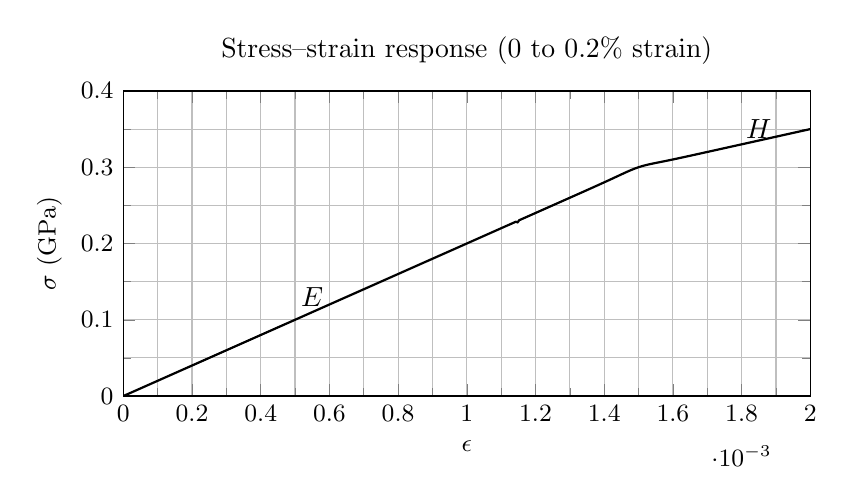
\begin{tikzpicture}
\begin{axis}[
    width=0.85\textwidth,
    height=0.45\textwidth,
    xlabel={$ \epsilon $},
    ylabel={$ \sigma \ \text{(GPa)} $},
    xmin=0, xmax=0.002,
    ymin=0, ymax=0.4,
    grid=both,
    minor tick num=1,
    ticklabel style={font=\small},
    label style={font=\small},
    title={Stress--strain response (0 to 0.2\% strain)}
]

% ---- Main stress–strain curve ----
\addplot[
    thick,
    domain=0:0.002,
    samples=400
] 
({x},
 {%
  (%
    (1 - (0.5*(1 + tanh((x - 0.0015)/5e-5))))*(200e9*x)
    + (0.5*(1 + tanh((x - 0.0015)/5e-5)))*(300e6 + 1e11*(x - 0.0015))
  )/1e9
 });

% ---- Elastic slope indicator (E) ----
\addplot[
    dashed,
    domain=0:0.0009,
    samples=2
]
({x},{(200e9*x)/1e9});

\node at (axis cs:0.00055,0.13) {$E$};

% ---- Post-yield slope indicator (H) ----
\addplot[
    dashed,
    domain=0.0016:0.002,
    samples=2
]
({x},{(300e6 + 1e11*(x - 0.0015))/1e9});

\node at (axis cs:0.00185,0.35) {$H$};

\end{axis}
\end{tikzpicture}
\caption{Stress--strain curve for a steel-like material, showing the elastic region and post-yield hardening over the strain range $0 \le \epsilon \le 0.002$.}
\end{figure}
%
%===========================================
Consider a uniform bar of length $L$ and cross-sectional area $A$, subjected to a constant axial force $P$.
The bar material exhibits a smooth nonlinear stress--strain relationship intended to mimic yielding
and post-yield hardening.

\subsection*{Constitutive law}

Let $\epsilon$ denote the axial strain and $\sigma(\epsilon)$ the axial stress.
Define the yield strain
\begin{equation}
\epsilon_y = \frac{\sigma_y}{E},
\end{equation}
and the smooth transition function
\begin{equation}
s(\epsilon) = \frac{1}{2}\left(1 + \tanh\!\left(\frac{\epsilon - \epsilon_y}{\delta}\right)\right),
\end{equation}
where $\delta>0$ controls the sharpness of the transition (smaller $\delta$ gives a sharper knee).

The stress--strain law is
\begin{equation}
\sigma(\epsilon) = (1-s(\epsilon))\,E\epsilon \;+\; s(\epsilon)\left[\sigma_y + H(\epsilon-\epsilon_y)\right].
\label{eq:sigma_smooth}
\end{equation}

\subsection*{Kinematics and equilibrium}

The axial strain is related to end displacement $u$ by
\begin{equation}
\epsilon = \frac{u}{L}.
\label{eq:strain_disp}
\end{equation}
Force equilibrium requires that the internal axial force equals the applied load:
\begin{equation}
P = A\,\sigma(\epsilon).
\label{eq:equil}
\end{equation}
%
Hence the displacement $u$ satisfies the nonlinear equation
\begin{equation}
f(u) = A\,\sigma\!\left(\frac{u}{L}\right) - P = 0.
\label{eq:f_u}
\end{equation}
where the stress $\sigma$ is given by Equation~\eqref{eq:sigma_smooth}.

\subsection*{(b) Newton's method formulation}

\begin{enumerate}[label=\arabic*.]
\item Compute $f'(u)$.
(\emph{Hint: use SymPy})
\item Write the Newton iteration
\begin{equation}
u^{(k+1)} = u^{(k)} - \frac{f\!\left(u^{(k)}\right)}{f'\!\left(u^{(k)}\right)}.
\label{eq:newton_update}
\end{equation}
\item Briefly explain the physical meaning of linearizing $f(u)$ about the current iterate.
\end{enumerate}

\subsection*{(c) Numerical solution}

Use Newton's method to solve for the displacement $u$ using the following data:

\begin{table}[h]
\centering
\caption{Material properties, geometry, and loading parameters used in the analysis.}
\begin{tabular}{lll}
\hline
\textbf{Symbol} & \textbf{Description} & \textbf{Value} \\
\hline
$E$          & Young's modulus                 & \SI{200}{GPa} \\
$\sigma_y$   & Yield stress                     & \SI{300}{MPa} \\
$H$          & Post-yield hardening modulus     & \SI{1e11}{Pa} \\
$\delta$     & Transition parameter             & $5\times10^{-5}$ \\
$L$          & Bar length                       & \SI{1}{m} \\
$A$          & Cross-sectional area             & \SI{1e-4}{m^2} \\
$P$          & Applied axial load               & \SI{35}{kN} \\
\hline
\end{tabular}
\end{table}

\begin{enumerate}[label=\arabic*.]
\item Use the linear-elastic solution as your initial guess:
\begin{equation}
u^{(0)} = \frac{PL}{AE}.
\end{equation}
\item Iterate until $|f(u)| < 10^{-8}$.
\item Report the converged displacement and the number of Newton iterations required.
\item Make a plot of $f(u)$ versus $u/L$ over $0 \le u/L \le 0.002$, and indicate the root on the plot.
\end{enumerate}

\subsection*{(d) Interpretation}

\begin{enumerate}[label=\arabic*.]
\item Compute the displacement predicted by linear elasticity.
\item Compare the linear and nonlinear solutions (numerically and in words).
\item Over the strain range considered (up to $0.2\%$), does the nonlinear response make the bar effectively stiffer or softer than linear elasticity?
\end{enumerate}

\section*{Submission Instructions}

Submit a single Jupyter notebook (\texttt{.ipynb}) containing:
\begin{itemize}
\item Your derivations (typeset using Markdown and LaTeX or cut and paste a screenshot or photo of handwritten work into markdown cell),
\item Your Newton implementation,
\item Numerical results,
\item Interpretation, including your plot.
\end{itemize}

\end{document}